\documentclass[10pt,a4paper]{article}
\usepackage[utf8]{inputenc}
\usepackage[T1]{fontenc}
\usepackage{amsmath}
\usepackage{amsfonts}
\usepackage{amssymb}
\usepackage[left=2cm,right=2cm,top=2cm,bottom=2cm]{geometry}
\author{Virginie Montalibet}
\title{Equation de Poisson et traitement d'image}
\begin{document}
\newpage
%%%%%%%%%%%%%%%%%%%%%%%%%%%%%%%%%%%%%%%%%%%%%%%%%%%%%%%%%%%
%                       EXPOSITION DU SUJET               %
%%%%%%%%%%%%%%%%%%%%%%%%%%%%%%%%%%%%%%%%%%%%%%%%%%%%%%%%%%%

Le traitement d'images est un ensemble de méthodes permettant d'étudier et de transformer une ou plusieurs images à l'aide de moyens mathématiques et numériques. Le principe du traitement d'images consiste à extraire certaines informations de celles-ci, afin de les étudier ou de les modifier.Il est utilisé dans beaucoup d'applications telles que l'amélioration du contraste, l'application d'un filtre(flou, lissage, changement de couleurs...) ou encore les détections et identifications d'objets par exemple. 

Aujourd'hui, nous nous intéressons à l'incrustation d'images. A partir de deux images, comment sélectionner une partie de la première et l'incruster de la manière la plus naturelle possible dans la seconde ? 
\newline
Afin d'éclaircir nos propos et d'identifier les problèmes que nous devons résoudre, voici un exemple de ce que nous souhaitons faire. Nous disposons des deux images présentées ci-dessous, l'image T(arget) et l'image S(ource). 
\newline
\begin{figure}[!htb]
   \begin{minipage}{0.48\textwidth}
     \centering
     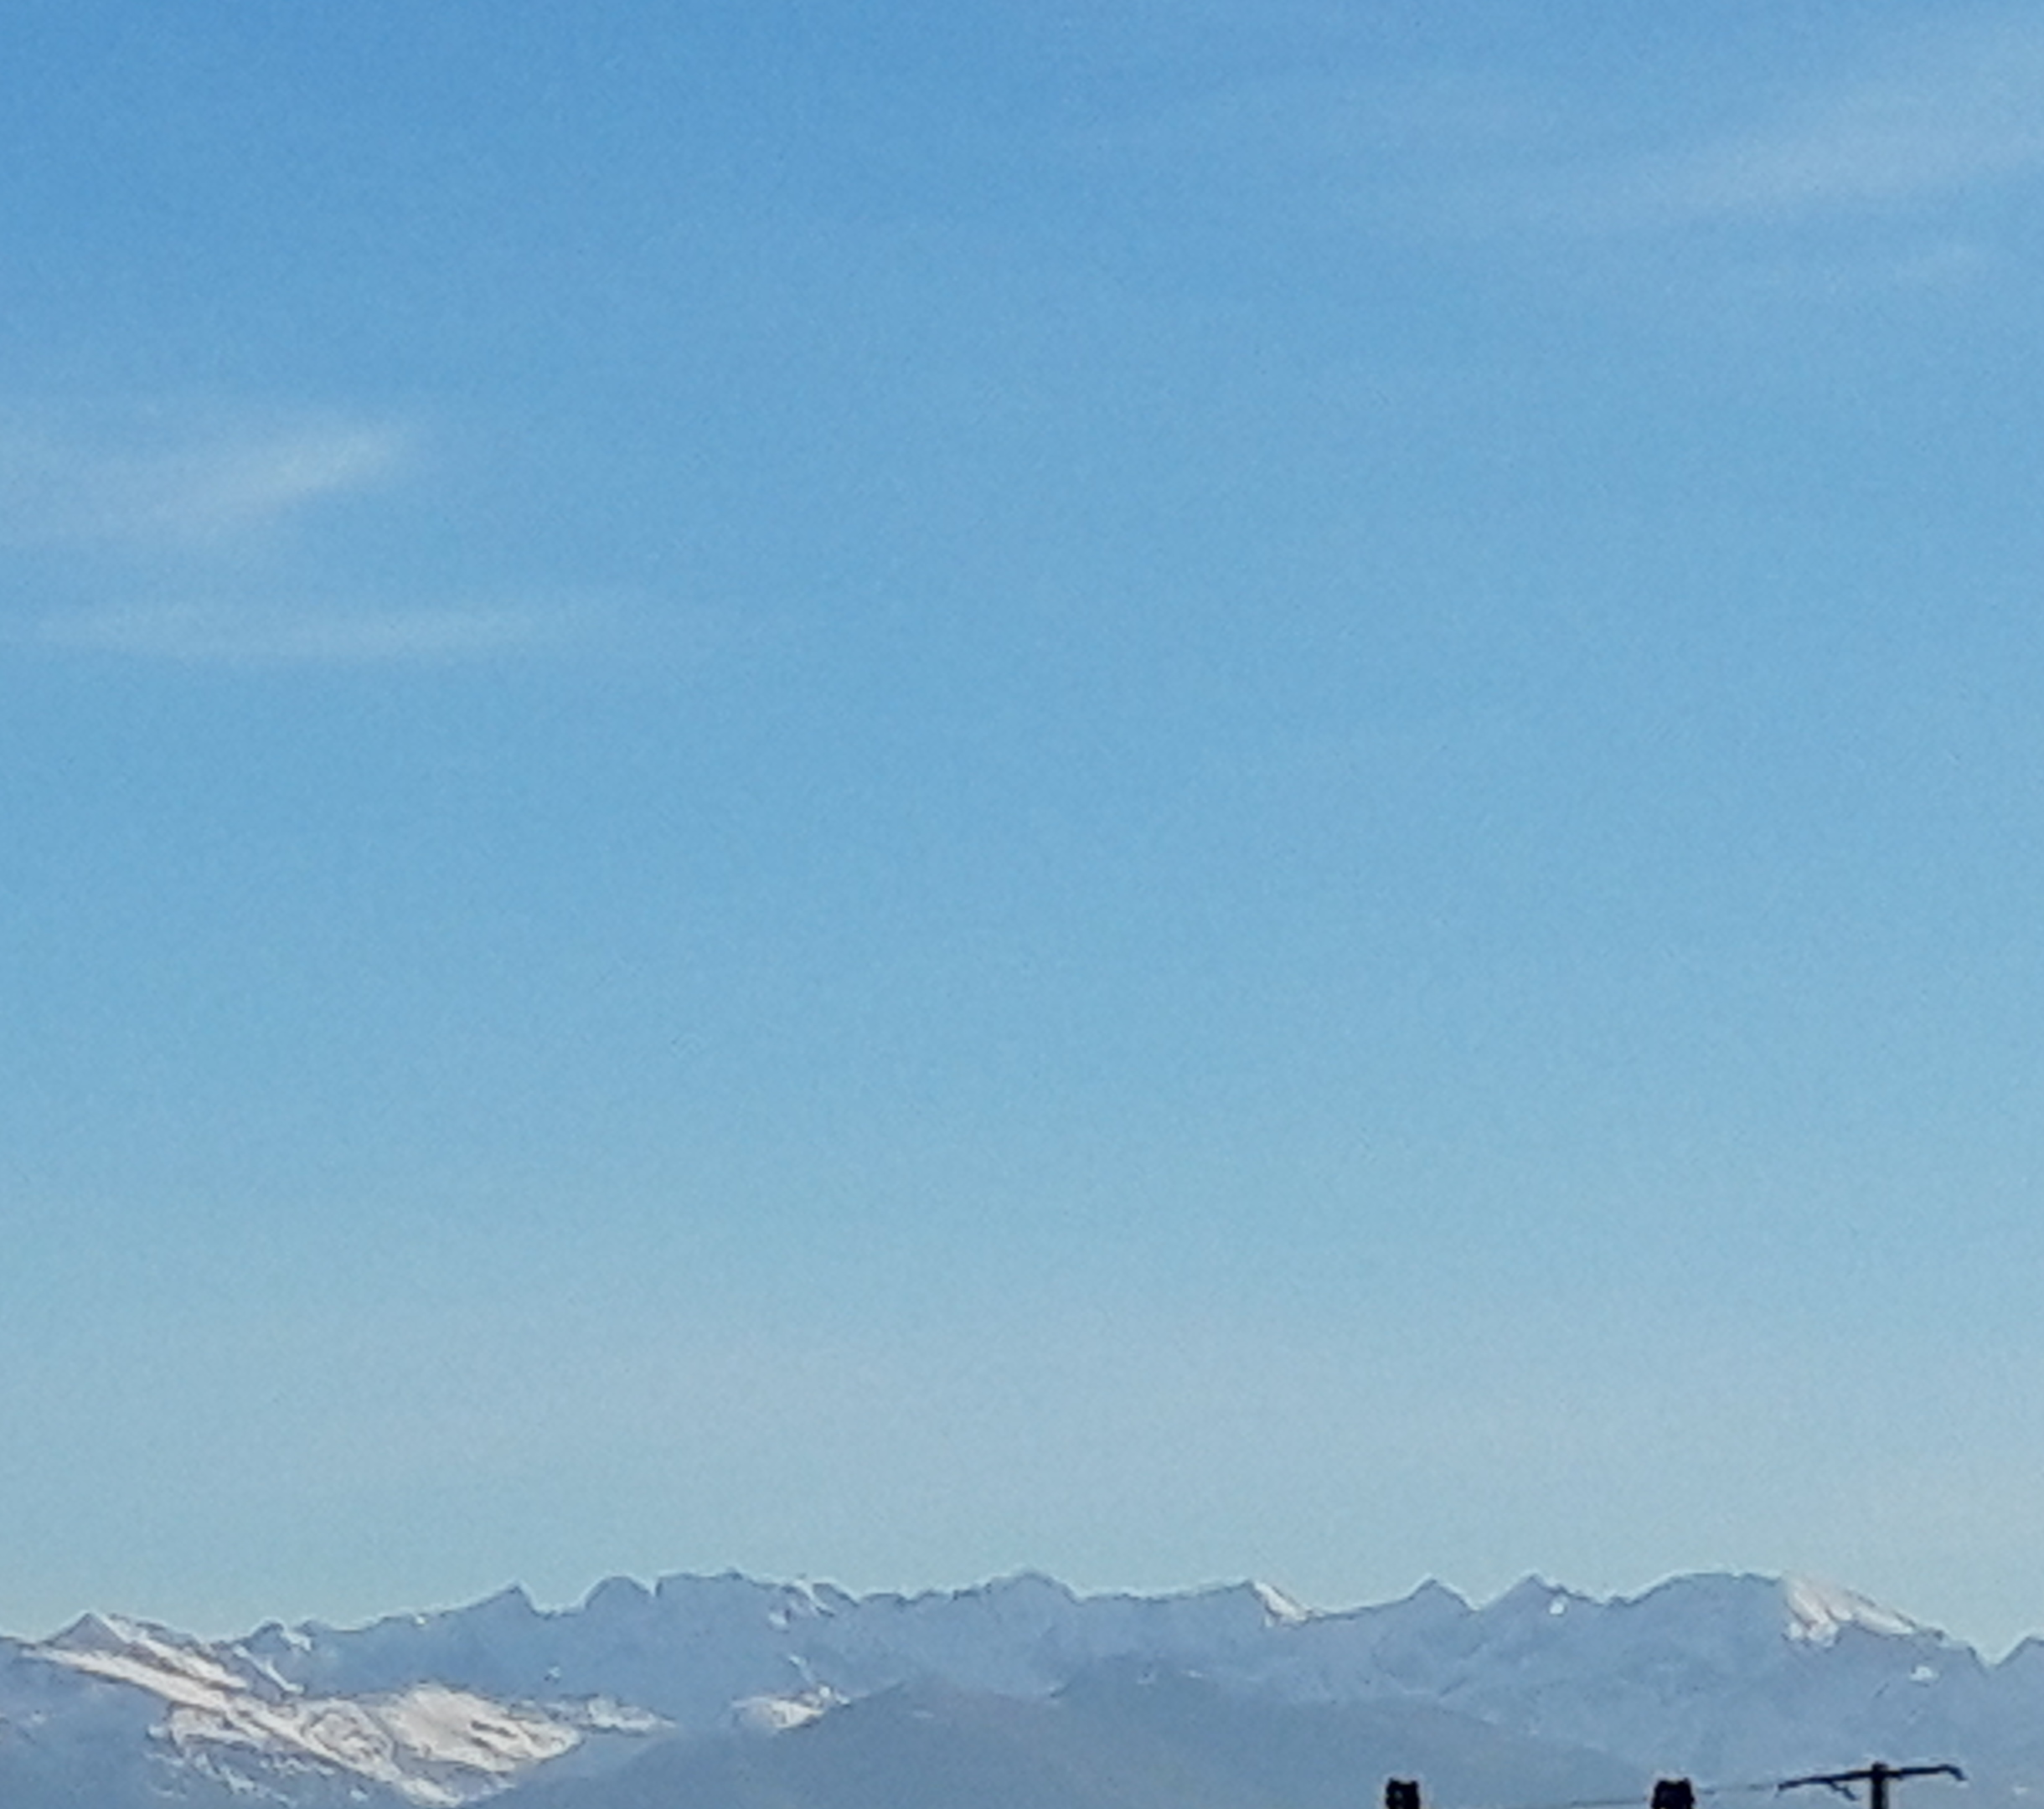
\includegraphics[scale=0.5]{Images/Montagne}
     \caption{Image T}
      \end{minipage}\hfill
   \begin{minipage}{0.48\textwidth}
     \centering
     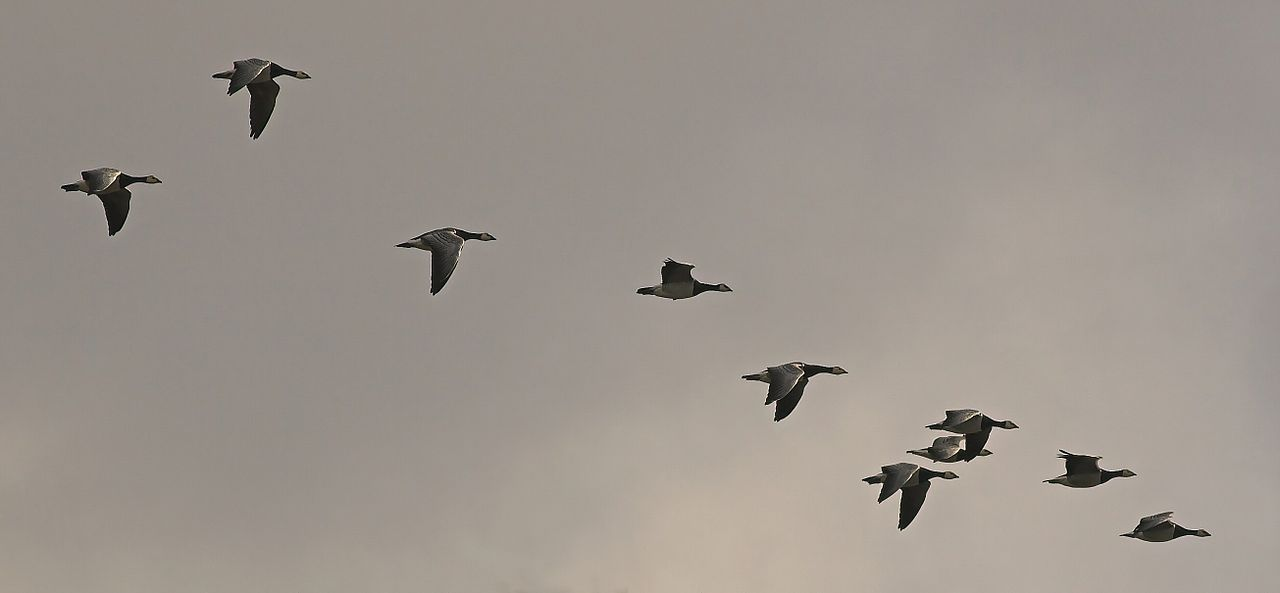
\includegraphics[width= 150pt]{Images/Oiseau.jpg}
     \caption{Image S}\label{Fig:Data2}
   \end{minipage}
\end{figure}

L'objectif est d'incruster toute ou partie de l'image S dans l'image T. Cela peut s'apparenter à un copier/coller ou encore à un clônage de la seconde image dans la première.
Le résultat que nous attendons pour une incrustation "réussie" est un résultat comme celui présenté ci-dessous : 
    
\begin{center}
\begin{figure}[!htb]
   \centering
     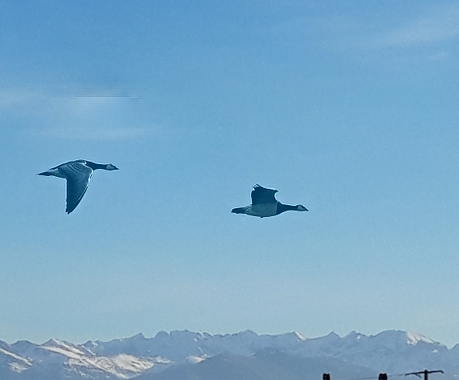
\includegraphics[width = 150pt]{Images/clonage_done.png}
     \caption{Image  finale attendue}
\end{figure}
\end{center}

Ce résultat semble naturel, les marques et bords de l'image collée sont très peu visibles, les oiseaux semblent faire partie de l'image.
Mais comment obtenir un tel résultat ? 
\newline
Reprenons nos deux images séparées, T et S.  La manière la plus simple de faire, serait de prendre une partie de l'image S,  puis de la transférer à l'endroit voulu dans l'image T. En effectuant cette manipulation voici l'image finale que nous devrions obtenir : 
\begin{center}
\begin{figure}[H]
     \centering
     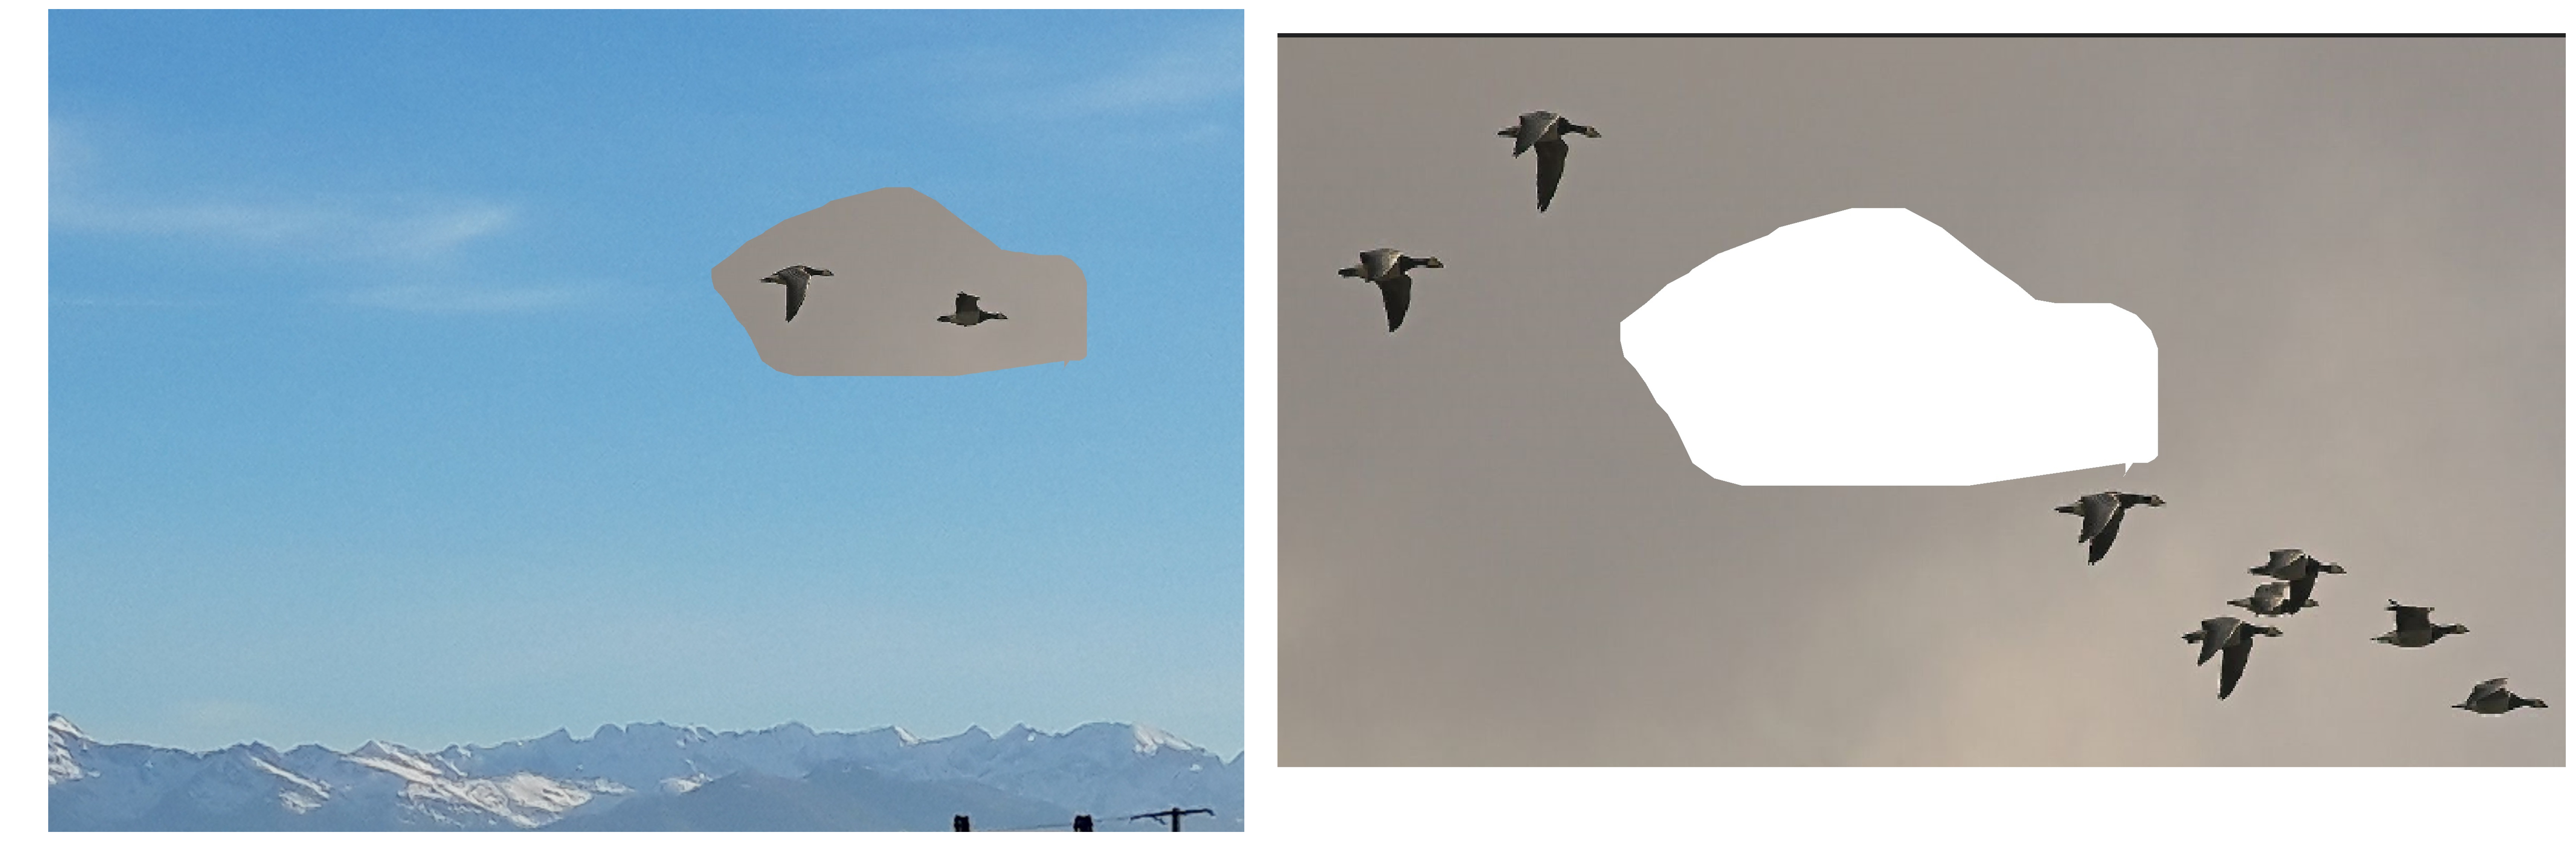
\includegraphics[width = 200pt]{Images/collage1.jpg}
     \caption{Simple copier/coller}
\end{figure}
\end{center}

Ce résultat n'est bien entendu pas convenable et bien loin de l'image finale attendue. Le découpage et la démarcation entre image originale et image collée sont beaucoup trop visibles, les couleurs ne sont pas les mêmes et incohérentes. Nous souhaitons obtenir un résultat beaucoup plus naturel comme écrit plus haut. Cette simple manipulation n'est donc pas suffisante pour effectuer le clônage d'une image dans une autre de manière "naturelle". \newline
L'objectif sera donc de faire disparaître ces problèmes de "démarcations" liés à un simple copier/coller. 

%%%%%%%%%%%%%%%%%%%%%%%%%%%%%%%%%%%%%%%%%%%%%%%%%%%%%%%%%%
%           TRADUCTION SOUS FORMES MATHEMATIQUES         %
%%%%%%%%%%%%%%%%%%%%%%%%%%%%%%%%%%%%%%%%%%%%%%%%%%%%%%%%%%

\subsection{Traduction du problème sous formes mathématiques.}

Considérons les deux images précédentes sous forme schématique. 
\begin{center}
    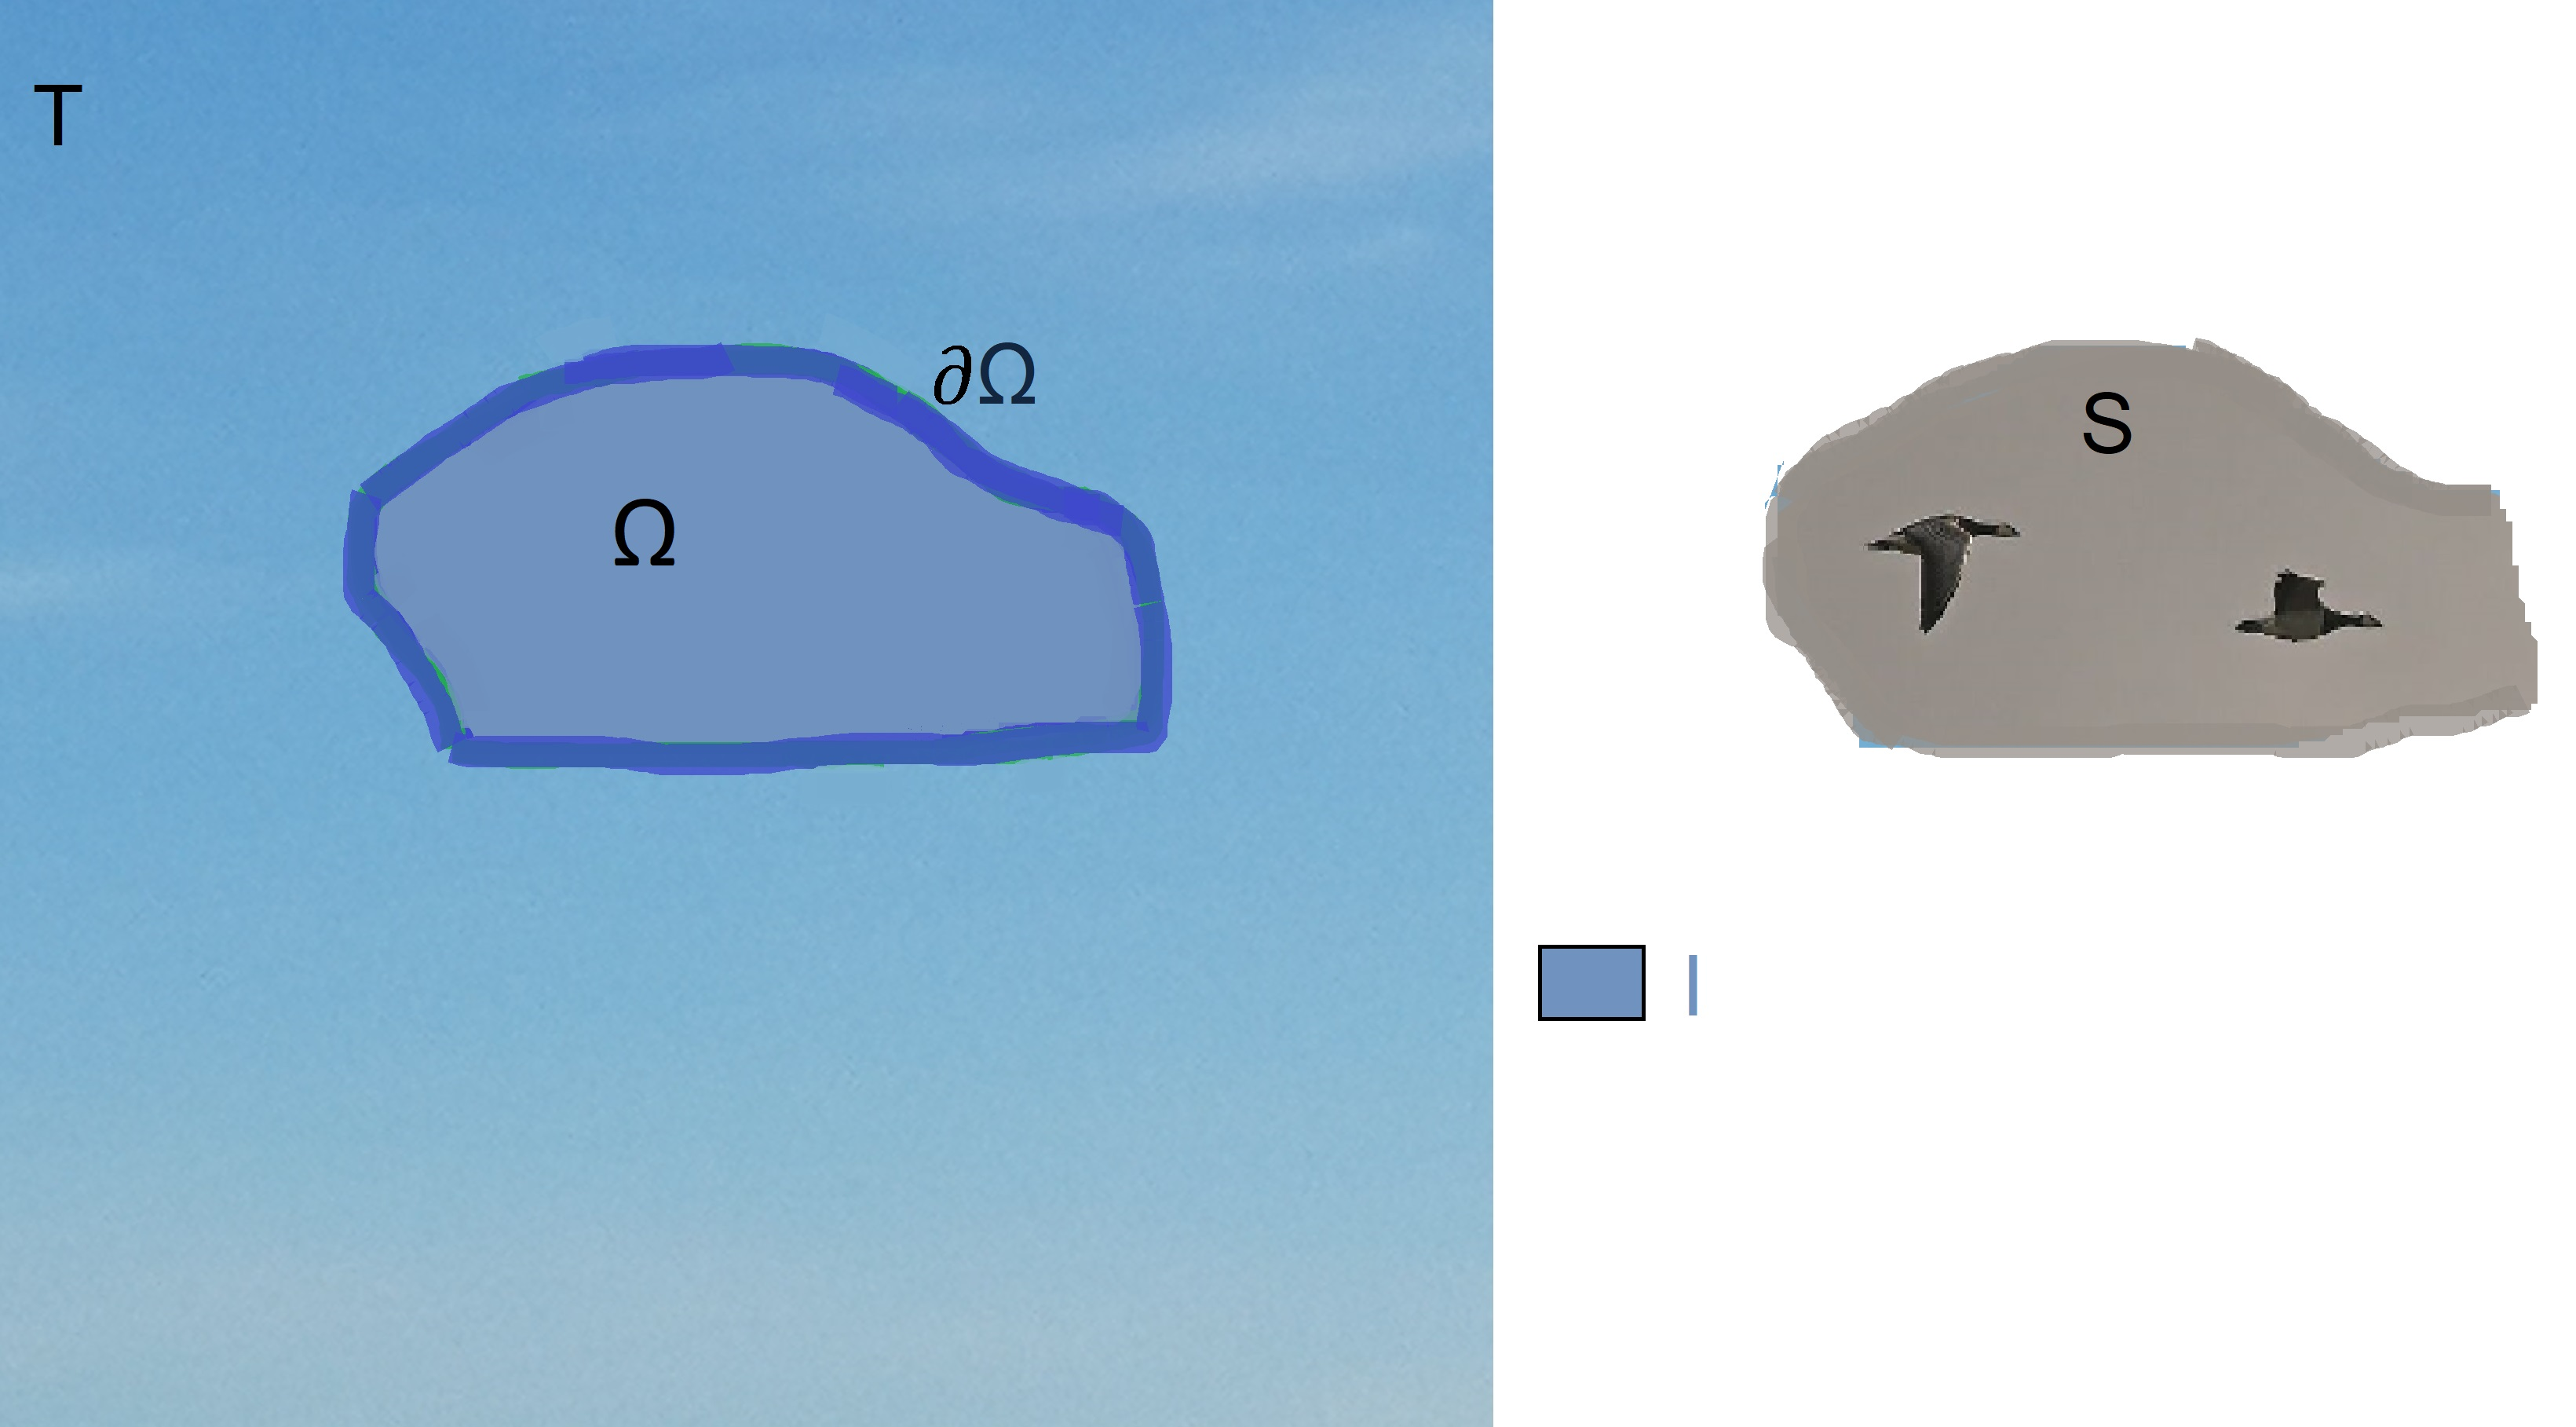
\includegraphics[width = 200pt]{Images/Schee.jpg}
\end{center}

Ici : 
\begin{itemize}
    \item T est l'image "Target", l'image destination, l'image sur laquelle s'effectuera le collage. 
    \item S est l'image "Source", l'image que nous souhaitons coller.
    \item $\Omega$ est la partie de l'image à copier/coller.
    \item $\partial \Omega$ est la frontière de $\Omega$.
    \item I est notre inconnue, la partie de l'image que nous ne connaissons pas et que nous souhaitons créer.
\end{itemize}

Notre objectif est donc de mixer deux images ensemble.  
Afin que l'image finale semble la plus cohérente possible, il faut apporter un certain nombre de modification à celle-ci. 

Ce que nous souhaitons déterminer ici, est la fonction $I$ de l'image de "fond". Mais alors une question se pose, pour que le rendu soit le meilleur possible, cette partie de l'image doit-elle être plus proche de l'image collée S, ou de l'image de fond T ? 
Pour répondre à cette question, reprenons le problème de départ. 
Nous souhaitons rendre le collage d'une image sur une autre le plus naturel qu'il soit. Il faut donc que le rendu final ne dénature aucune des deux images sélectionnées au départ. En effet, nous devons garder les détails de l'image collée S, ne pas modifier les variations qu'elle pourrait posséder, les contours des objets qu'elle possède, par exemple. Il faut donc que les variations présentes dans $I$ soient presque identiques à celles de S. Mathématiquement, cela revient à dire que les gradients de $I$ et S soient très proches, voir identiques. Ce problème s'écrit de la manière suivante :
\begin{center}
    $$ min \iint_\Omega || \nabla I_{x,y} - \nabla S_{x,y}||^2 dxdy$$
\end{center} 

Mais les démarcations entre l'image collée  et l'image de fond, T, ne doivent pas non plus être visibles, il faut donc que les pixels se situant sur cette partie là, i.e $\partial \Omega$, soient le plus proches possible de T .  Mathématiquement cela revient à écrire : 
\begin{center}
    $I_{(x,y)} = T_{x,y} \ sur\ \partial \Omega$
\end{center}

Répondre au problème implique donc de résoudre un problème variationnel classique auquel des conditions sur le bord sont ajoutées. 
Réécrivons le problème mathématique que nous cherchons à résoudre :  

\begin{center}
\begin{equation*}
\left\{
\begin{aligned}
 min \iint_\Omega || \nabla I_{x,y} - \nabla S_{x,y}||^2 dxdy\\
 I_{(x,y)} = T_{x,y} \ sur\ \partial \Omega
\end{aligned}
\right.
\end{equation*}
\end{center}

Notons $g(\nabla f, v)$ la fonction  : 
$$g(\nabla f, v) =\int ||\nabla f-v ||^2$$ 
\newline
Rappelons qu'ici $\nabla f$ est le gradient de f que l'on peut noter $\nabla f = (\frac{\partial f}{\partial x} \frac{\partial f}{\partial y})^T$ et v est un vecteur que l'on notera $v = (v_x, v_y)$. 
Ainsi nous pouvons réecrire g sous la forme suivante : 
$$g(\nabla f, v) =\int( (\frac{\partial f}{\partial x}-v_x)^2+(\frac{\partial f}{\partial y}-v_y)^2) $$\newline

Mais la fonction f qui minimise le problème posé,  satisfait l'équation d'Euler-Lagrange ci-dessous : 

\begin{equation*}
    \frac{\partial g}{\partial f}-\frac{d}{dx}\frac{\partial g}{\partial f   }-\frac{d}{dy}\frac{\partial g}{\partial f}= 0 \\
\end{equation*}
\begin{equation*}
    \frac{\partial g}{\partial f}-\frac{d}{dx}\frac{\partial g}{\partial f}-\frac{d}{dy}\frac{\partial g}{\partial f}= 0 \\
\end{equation*}

\begin{equation*}
    2\times()
\end{equation*}

\begin{center}
    
\includegraphics[width = 100pt]{Images/EXPLICATIONS_needed.png}
\end{center}

\begin{equation*}
    2(\frac{\partial^2 f}{\partial x^2}-\frac{\partial v_x}{\partial x}+\frac{\partial^2 f}{\partial y^2}\frac{\partial v_y}{\partial y}) = 0 ?
\end{equation*}

\begin{equation}
    \Delta f = div v
\end{equation}



Résoudre ce problème variationnel est équivalent à résoudre l'équation de poisson avec conditions aux bords de Dirichlet, suivante :
\begin{center}
    \begin{equation*}
        \left\{
        \begin{aligned}
         \Delta I = \Delta S  \ sur \  \Omega \\
          I = T \ sur \  \partial \Omega
        \end{aligned}
        \right.
    \end{equation*}
\end{center}

Nous devons donc faire en sorte que les laplaciens de I et S soient les mêmes.Nous verrons deux approches afin de résoudre cette équation, la première utilisant des discrétisations, la seconde la méthode de Fourier. 


\end{document}}